\chapter{System}
Dieses Kapitel bietet eine grobe Übersicht über das ganze System, um die Zusammenhänge zwischen einzelnen Komponenten aufzuzeigen.
Auf einzelne Komponenten wird in den folgenden Kapiteln genauer eingegangen.


\section{Schematische Übersicht}
Das \textit{Zybo} beinhaltet neben dem FT2232 auch noch diverse I/O-Peripherien, die in einer \textit{deep}-Applikation genutzt werden können.
Der FT2232-Chip auf dem \textit{Zybo} übernimmt zwei verschiedene Funktionen.
Einerseits wird er als USB zu UART Brücke verwendet, damit man mit dem Windows PC einfach eine serielle Verbindung mit dem Prozessor aufbauen kann, andererseits fungiert er als Brücke zum blauen JTAG-Bus.
Das bedeutet, er erhält Befehle von OpenOCD über USB und übersetzt diese elektrisch und auch logisch für das JTAG Interface.

In Abbildung \ref{fig:UebersichtDebuggerToolchain} ist das ganze System abgebildet.
Auf dem \textit{Windows PC} wird die \textit{deep}-Applikation in Eclipse geschrieben, kompiliert und debuggt.
Plugins erweitern Eclipse um die notwendige Funktionen, die für die Entwicklung von \textit{deep}-Applikationen notwendig sind.
Es sind beide Debug Toolchains, die ''klassische'' Abatron-Toolchain und die neue OpenOCD-Toolchain, in dieser Übersicht abgebildet.

Bei der \textit{Abatron-Toolchain} wird das \textit{Abatron BDI3000} über die rote TCP/IP-Verbindung angesprochen.
Das BDI kommuniziert dann über die blaue JTAG-Verbindung direkt mit dem Zynq-Chip.

Die grünen Pfeile zeigen den Kommunikationsweg für die beiden neuen OpenOCD-Toolchains.
OpenOCD bildet zusammen mit der richtigen Hardware, hier ist es der FT2232-Chip, einen kompletten Debugger und ist somit eine Alternative zum BDI.
OpenOCD stellt einen \textit{gdb}-Server und auch ein CLI (\textit{Command Line Interface}) zur Verfügung.
% referenz zu openOCDInterface
Das neue Eclipse-Plugin \textit{openOCDInterface} verwendet das CLI über den TCP/IP-Port 4444 (gestrichelter, grüner Pfeil) und bildet so die \textit{CLI-OpenOCD-Toolchain}.
Die \textit{gdb-OpenOCD-Toolchain} kommuniziert mit dem \textit{gdb}-Server von OpenOCD mit dem \textit{gdb}-Protokoll über den TCP/IP-Port 3333 (grüner Pfeil mit Strich-Punkt-Muster).
OpenOCD verwendet dann den \textit{WinUSB}-Treiber um mit dem FT2232-Chip zu kommunizieren.
Der FT2232 verwendet den selben, blauen JTAG-Bus wie das BDI3000 als Verbindung mit dem Zynq.

\begin{figure}[htbp]
	\centering
		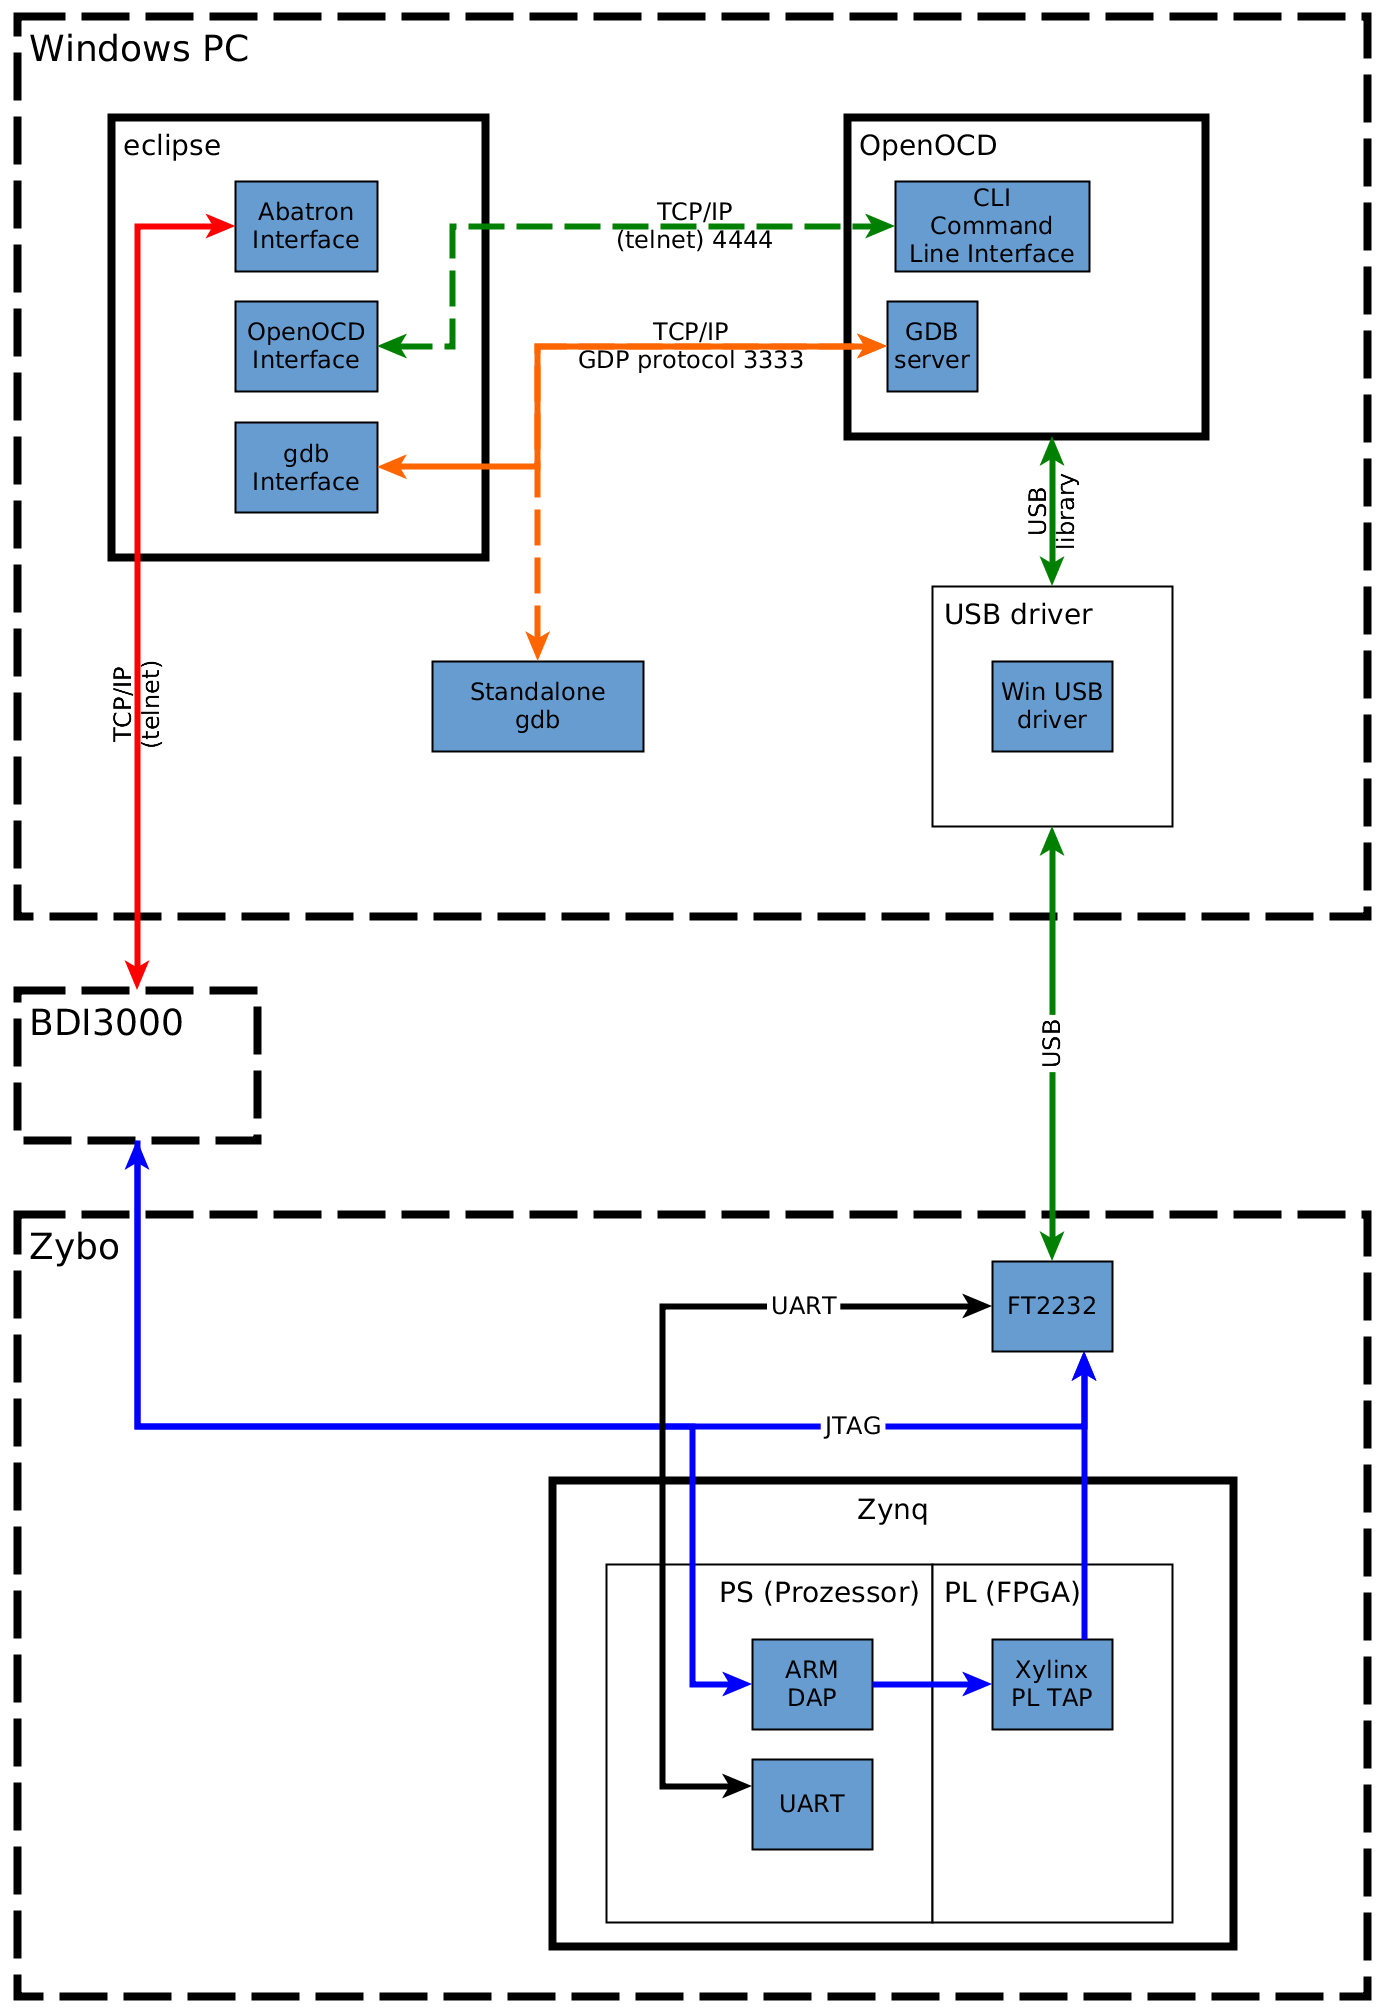
\includegraphics[width=\textwidth,height=\textheight,keepaspectratio]{graphs/embeddedDebuggerToolchain.png}
	\caption{Systemübersicht Debugger Toolchain}
	\label{fig:UebersichtDebuggerToolchain}
\end{figure}


\section{Debugger Toolchains}
Im Folgenden werden die drei verschiedenen Toolchains genauer erklärt.

\subsection{Abatron-Toolchain}
Die \textit{Abatron-Toolchain} benötigt weder OpenOCD noch den FT2232, dafür aber das teure BDI3000.
Diese ''klassische'' Toolchain wird für die Entwicklung von \textit{deep}-Applikationen für den PowerPC verwendet.
In dieser Arbeit wird sie aber nicht verwendet.
% TODO: Schema


\subsection{CLI-OpenOCD-Toolchain}
Das teure BDI wird für diese Toolchain nicht  benötigt.
% verbessern: satzbau
Da das CLI\footnote{Command Line Interface} von OpenOCD aber sehr ähnlich ist wie das CLI des BDI, ist eine Portierung der bestehenden \textit{Abatron-Toolchain} in die neue \textit{CLI-OpenOCD-Toolchain} relativ einfach.
Die \textit{CLI-OpenOCD-Toolchain} lehnt sich deshalb sehr stark an die bestehende \textit{Abatron-Toolchain} an.
% Die bestehende Toolchain für den PPC ist nicht auf der offiziellen \textit{deep}-Homepage dokumentiert.

Mit dieser Toolchain ist \textit{Sourcecode-Debugging} aber nicht möglich.
Das bedeutet, es ist nicht möglich im Sourcecode Breakpoints zu setzten oder durch einzelne Zeilen im Sourcecode zu steppen wie man es von Debuggern, wie dem \textit{gdb}, gewohnt ist.
% TODO wirklich target commands?
Bestehende Möglichkeiten aus der alten \textit{Abatron-Toolchain}, wie \textit{Target Commands}, bleiben aber erhalten.
% TODO: Schema

Im Kapitel \ref{section:CLI-OpenOCD-Toolchain} wird diese Toolchain genauer beschrieben.


\subsection{\textit{gdb}-OpenOCD-Toolchain}
In der \textit{gdb-OpenOCD-Toolchain} wird, wie bei der obigen Toolchain, ebenfalls die OpenOCD-Software und der FT2232-Chip verwendet.
Es wird aber nicht mehr ein Interface bestehend auf der ''klassischen'' Abatron Toolchain verwendet, sondern es wird direkt der bekannte \textit{gdb}-Debugger verwendet.
% Dadurch kann \textit{Sourcecode-Debugging} direkt in Eclipse eingesetzt werden.
Dadurch kann auch \textit{Sourcecode-Debugging} verwendet werden.
% günstige hardware
% TODO: Schema
% TODO: Verweis

Im Kapitel \ref{chapter:Der-gdb-Debugger} wird diese Toolchain detailliert beschrieben.
